\documentclass{article}
\usepackage[utf8]{inputenc}
\usepackage{graphicx}
\usepackage{amsmath, amssymb}
\title{Simulation - chapter 5, even exercises}
\author{Pinak Mandal}
\date{}

\begin{document}

\subsection*{Problem 2}
The distribution function is given by
\begin{align*}
  F(x) = \begin{cases}
            \frac{(x-2)^2}{4}, & 2\le x\le 3 \\
            \frac{1}{4} + \frac{(x-3)(9-x)}{12}, & 3\le x\le 6
        \end{cases}
\end{align*}
The inverse to which is given by
\begin{align*}
  F^{-1}(y) = \begin{cases}
                2(\sqrt{y}+1), & 0\le y\le \frac{1}{4}\\
                6-2\sqrt{3(1-y)}, & \frac{1}{4}\le y\le 1
              \end{cases}
\end{align*}
$1000$ samples generated with inverse transform algorithm yield the following result.
\begin{figure}[h!]
    \centering
    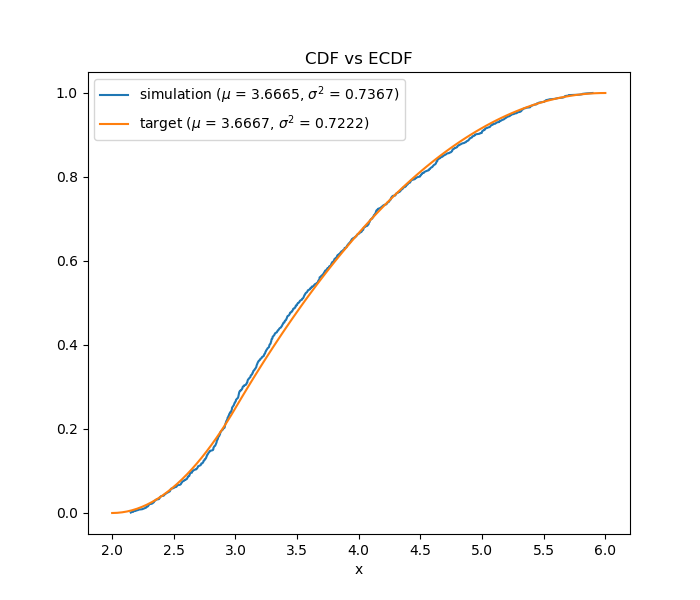
\includegraphics[width=\linewidth]{../images/p2_1000.png}
    \caption{distribution comparison}
\end{figure}
\newpage

\subsection*{Problem 4}
\begin{align*}
  F^{-1}(y) = \left[-\frac{\log(1-y)}{\alpha}\right]^{\frac{1}{\beta}}
\end{align*}
The pdf is given by
\begin{align*}
  f(x) = \alpha\beta\,x^{\beta-1}\exp(-\alpha x^{\beta})
\end{align*}
The mean is $\frac{1}{\sqrt[\beta]{\alpha}}\Gamma\left(1+\frac{1}{\beta}\right)$ and the variance is $\frac{1}{\sqrt[\beta]{\alpha^2}}\left[\Gamma\left(2+\frac{1}{\beta}\right)-\Gamma\left(1+\frac{1}{\beta}\right)^2\right]$.
$1000$ samples generated with inverse transform algorithm yield the following result.
\begin{figure}[h!]
    \centering
    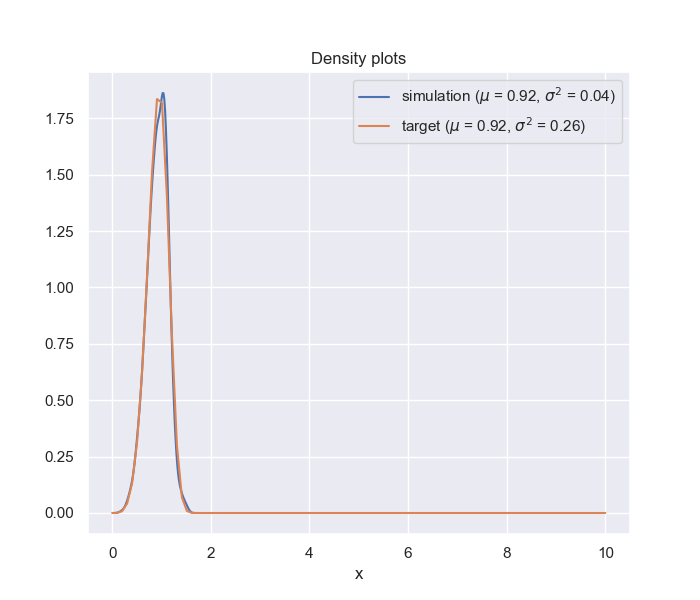
\includegraphics[width=\linewidth]{../images/p4_density_it_1_5_1000.png}
    \caption{density comparison for $\alpha = 1,\,\beta = 5$}
\end{figure}
\newpage

\subsection*{Problem 6}
The inverse of the cdf is given by
\begin{align*}
  F^{-1}(y) = -\log(1-cy), \;\; c = 1 - e^{-0.05}
\end{align*}
Mean of the target distribution is given by,
\begin{align*}
  \frac{1-1.05e^{-0.05}}{1-e^{-0.05}}
\end{align*}
$1000$ samples generated with inverse transform algorithm yield the following result.
\begin{figure}[h!]
    \centering
    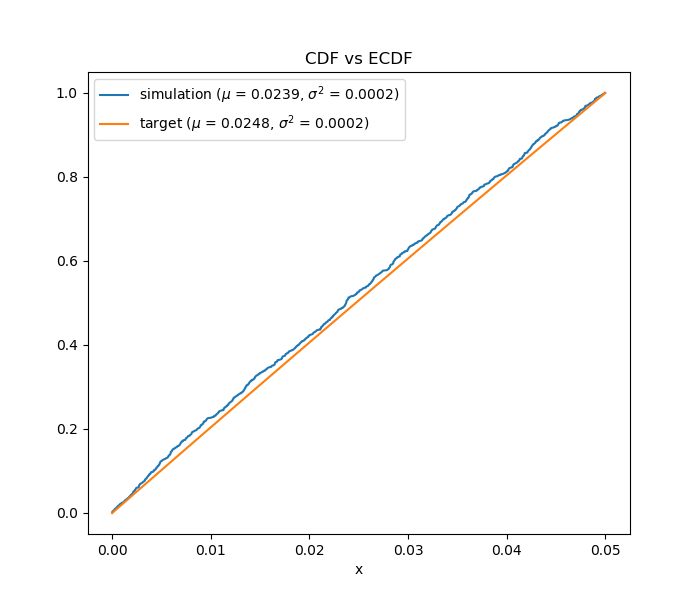
\includegraphics[width=\linewidth]{../images/p6_dist_it_1000.png}
    \caption{distribution comparison}
\end{figure}
\newpage

\subsection*{Problem 8(a)}
The inverse of $F_{i}(x)$ is given by
\begin{align*}
  F_{i}^{-1}(y)=y^{\frac{1}{2i-1}}, \;\; i=1,2,3
\end{align*}
$1500$ samples generated with composition method yield the following result.
\begin{figure}[h!]
    \centering
    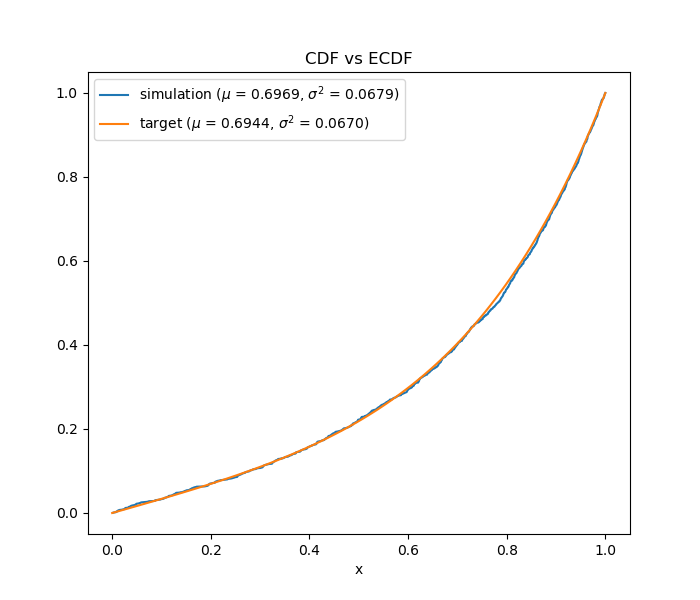
\includegraphics[width=\linewidth]{../images/p8a_dist_incomp_1500.png}
    \caption{distribution comparison}
\end{figure}
\newpage

\subsection*{Problem 8(b)}
Our setup is as follows.
\begin{align*}
  F_1(x) &= 1-e^{-2x},\;\; 0< x< \infty\\
  F_2(x) &= \begin{cases}
              x, & 0< x< 1\\
              1, & 1\le x<\infty
            \end{cases}\\
  F(x) &= \frac{1}{3}F_{1}(x) + \frac{2}{3}F_{2}(x)\\
\end{align*}
$1500$ samples generated with composition method yield the following result.
\begin{figure}[h!]
    \centering
    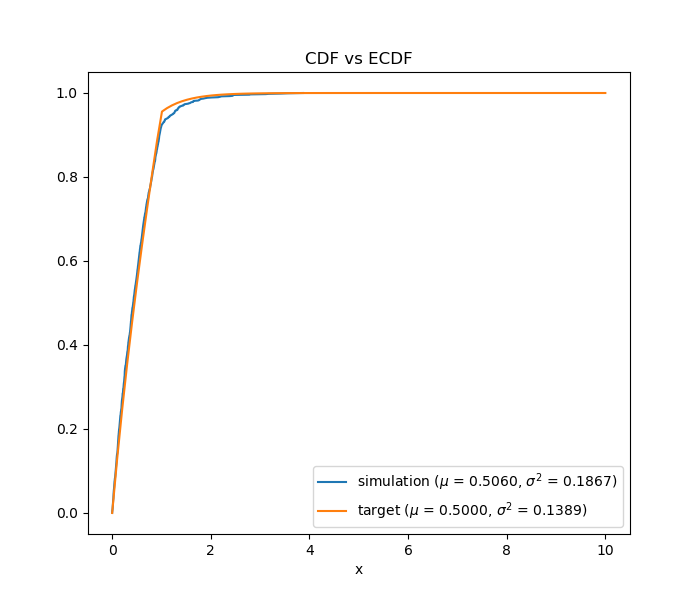
\includegraphics[width=\linewidth]{../images/p8b_dist_incomp_1500.png}
    \caption{distribution comparison}
\end{figure}
\newpage

\subsection*{Problem 8(c)}
Our setup is as follows. The probability weights have been generated randomly.
\begin{align*}
  F(x) = 0.21339248x + 0.2047535x^2 +  0.27419785x^3 + 0.01031662x^4 + 0.29733956 x^5
\end{align*}
$1500$ samples generated with composition method yield the following result.
\begin{figure}[h!]
    \centering
    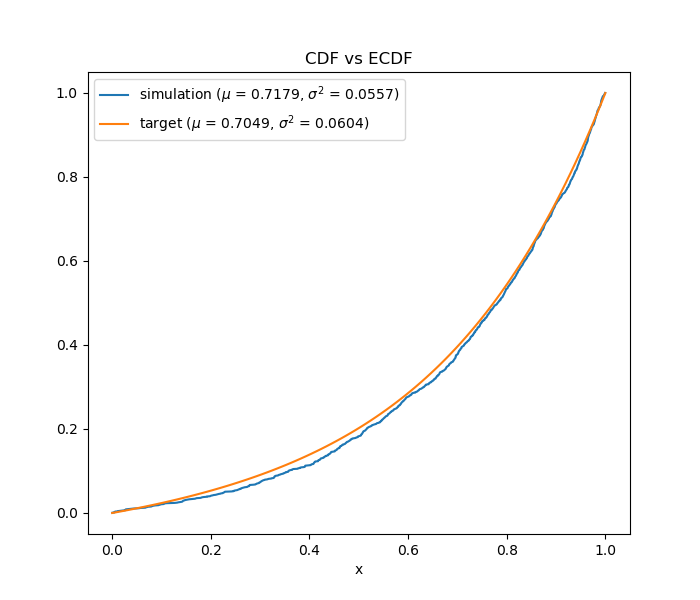
\includegraphics[width=\linewidth]{../images/p8c_dist_incomp_1500.png}
    \caption{distribution comparison}
\end{figure}
\newpage

\end{document}
